%%%%% Beginning of preamble %%%%%

\documentclass[12pt]{article}  %What kind of document (article) and what size
\usepackage[document]{ragged2e}


%Packages to load which give you useful commands
\usepackage{graphicx}
\usepackage{amssymb, amsmath, amsthm}
\usepackage{fancyhdr}
\usepackage[linguistics]{forest}
\usepackage{enumerate}
\usepackage[margin=0.75in]{geometry} 
\pagestyle{fancy}
\fancyhf{}
\lhead{MA 750: HW4}
\rhead{Benjamin Draves}


\renewcommand{\headrulewidth}{.4pt}
\renewcommand{\footrulewidth}{0.4pt}


\topmargin = -0.4 in
\parskip = 0.2in

%%%%%%%%%%new commands%%%%%%%%%%%%
\newcommand{\N}{{\mathbb{N}}}
\newcommand{\Z}{{\mathbb{Z}}}
\newcommand{\R}{{\mathbb{R}}}
\newcommand{\Q}{{\mathbb{Q}}}
\newcommand{\e}{{\epsilon}}
\newcommand{\del}{{\delta}}
\newcommand{\m}{{\mid}}
\newcommand{\infsum}{{\sum_{n=1}^\infty}}
\newcommand{\la}{{\langle}}
\newcommand{\ra}{{\rangle}}
\newcommand{\E}{{\mathbb{E}}}
\newcommand{\V}{{\mathbb{V}}}

%defines a few theorem-type environments
\newtheorem{theorem}{Theorem}
\newtheorem{corollary}[theorem]{Corollary}
\newtheorem{definition}{Definition}
\newtheorem{lemma}[theorem]{Lemma}
%%%%% End of preamble %%%%%

\begin{document}

\begin{enumerate}
\item 
\begin{enumerate}
\item 
\begin{align*}
\int_{-1}^{p}B(w,p)dw &= \int_{-1}^{p}\frac{a_2(p)-a_1(p)w}{a_0(p)a_2(p)-a_1^2(p)}K(w)dw\\
&= \frac{1}{a_0(p)a_2(p) - a_1^2(p)}\bigg[a_2(p)\int_{-1}^{p}K(w)dw - a_1(p)\int_{-1}^{p} wK(w)dw\bigg]\\
&=  \frac{1}{a_0(p)a_2(p) - a_1^2(p)}\left(a_2(p)a_0(p) - a_1^2(p)\right)\\
&= 1
\end{align*}

\begin{align*}
\int_{-1}^{p}wB(w,p)dw &= \int_{-1}^{p}\frac{a_2(p)w-a_1(p)w^2}{a_0(p)a_2(p)-a_1^2(p)}K(w)dw\\
&= \frac{1}{a_0(p)a_2(p) - a_1^2(p)}\bigg[a_2(p)\int_{-1}^{p}wK(w)dw - a_1(p)\int_{-1}^{p} w^2K(w)dw\bigg]\\
&=  \frac{1}{a_0(p)a_2(p) - a_1^2(p)}\left(a_2(p)a_1(p) - a_1(p)a_2(p)\right)\\
&= 0
\end{align*}

\begin{align*}
\E(\hat{f}_h(x)) &= \frac{1}{nh}\sum_{i=1}^{n}\E\Big[B\left(\frac{x-X_i}{h}\right)\Big]\\
&= \frac{1}{h}\E\Big[B\left(\frac{x-w}{h}\right)\Big]\\
&= \frac{1}{h}\int B\left(\frac{x-w}{h}\right)f(w)dw\\
&\overset{z-sub}{=}\int B(z)f(x-zh)dz\\
&\overset{Taylor}{=}\int B(z)\Big\{f(x) - zhf'(x) + \frac{z^2h^2}{2}f''(x) +O(h^2)\Big\}dz\\
&= f(x) + f''(x)\frac{h^2}{2}\mu_2(B) + O(h^2)
\end{align*}

Therefore the first term in the bias is given by $$f''(x)\frac{h^2}{2}\mu_2(B)$$
\item We first find the polynomials, $a_0(p)$, $a_1(p)$, and $a_2(p)$. Then we will use these to write the form of the boundary kernel using the Epanechnikov kernel. 

\begin{align*}
a_0(p) &= \int_{-1}^{p}\frac{3}{4}(1-t^2)dt = \frac{3}{4}\left(p-\frac{p^3}{3} +\frac{2}{3}\right)\\
a_1(p) &= \int_{-1}^{p}\frac{3t}{4}(1-t^2)dt = \frac{3}{4}\left(\frac{p^2}{2}-\frac{p^4}{4} -\frac{1}{4}\right)\\
a_2(p) &= \int_{-1}^{p}\frac{3t^2}{4}(1-t^2)dt = \frac{3}{4}\left(\frac{p^3}{3}-\frac{p^5}{5} +\frac{2}{15}\right)\\
\end{align*}

This gives the formula for boundary kernel. 

\begin{align*}
B(t,p) &= \frac{a_2(p)-a_1(p)t}{a_0(p)a_2(p)-a_2(p)^2}K(t)I_{[-1,p]}(t)\\
&= \frac{\frac{p^3}{3}-\frac{p^5}{5} +\frac{2}{15} - t\left(\frac{p^2}{2}-\frac{p^4}{4} -\frac{1}{4}\right)}{\frac{3}{4}\left(\frac{p^3}{3}-\frac{p^5}{5} +\frac{2}{15}\right)\left(p-\frac{p^3}{3} +\frac{2}{3}\right)-\frac{3}{4}\left(\frac{p^2}{2}-\frac{p^4}{4} -\frac{1}{4}\right)^2}(1-t^2)I_{[-1,p]}(t)
\end{align*}

\begin{figure}[h]
\centering
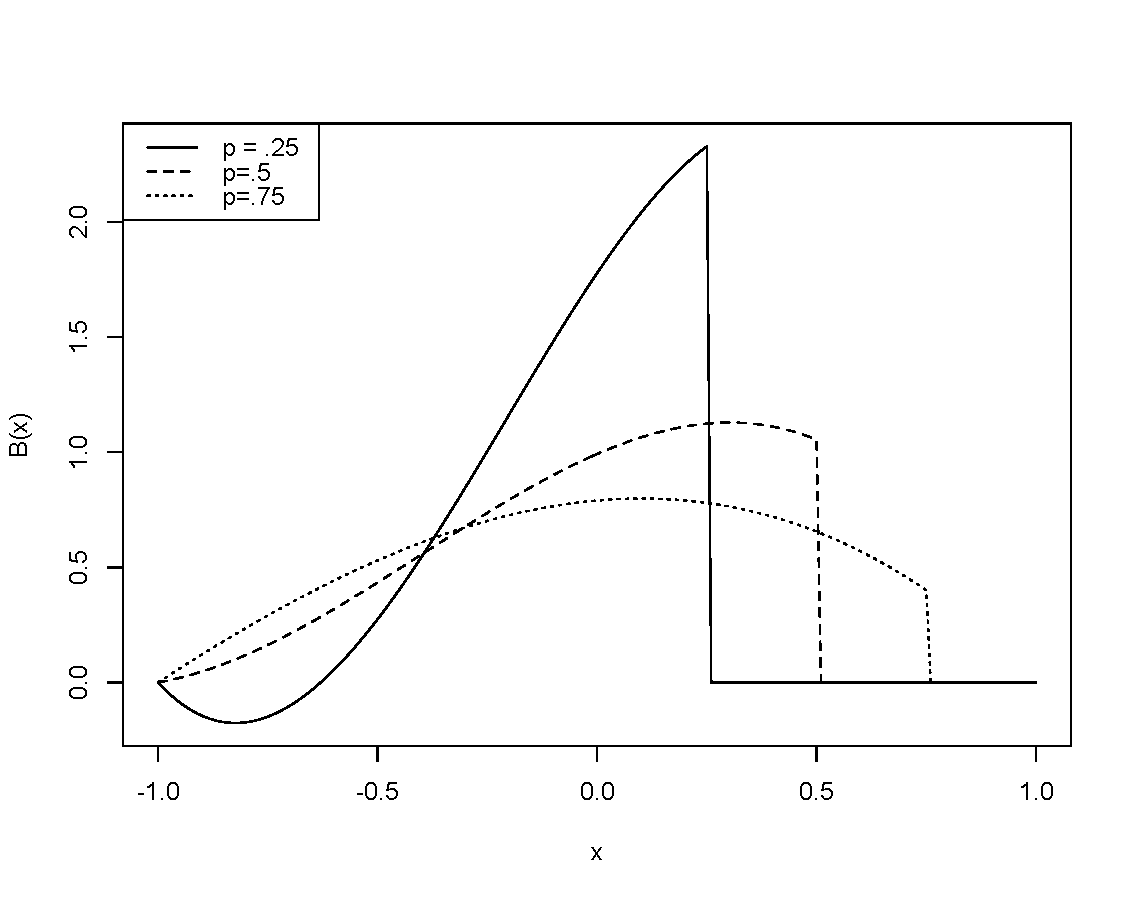
\includegraphics[width = 0.7\textwidth]{p1.pdf}
\end{figure}


\end{enumerate}
\item 
\begin{enumerate}
\item 
\begin{align*}
\int K_4(t)dt &= \int \frac{s_4-s_2t^2}{s_4-s_2^2}K(t)dt\\
&= \frac{1}{s_4 -s_2^2}\bigg[s_4\int K(t)dt - s_2\int t^2K(t)dt\bigg]\\
&= \frac{1}{s_4 -s_2^2} (s_4 -s_2^2)\\
&= 1
\end{align*}
\item Recall that $K(t)$ is a symmetric function, so $s_{2n+1} = 0$ for any $n = 0,1,2,\ldots$. That is $s_k = 0$ for any $k$ odd. 
\begin{align*}
\int tK_4(t)dt &= \frac{1}{s_4-s_2^2}\bigg[s_4\int tK(t)dt-s_2\int t^3K(t)dt\bigg] = \frac{1}{s_4-s_2^2}(s_4s_1 - s_2s_3) = 0\\
\int t^2K_4(t)dt &= \frac{1}{s_4-s_2^2}\bigg[s_4\int t^2K(t)dt-s_2\int t^4K(t)dt\bigg] = \frac{1}{s_4-s_2^2}(s_4s_2 - s_2s_4) = 0\\
\int t^3K_4(t)dt &= \frac{1}{s_4-s_2^2}\bigg[s_4\int t^3K(t)dt-s_2\int t^5K(t)dt\bigg] = \frac{1}{s_4-s_2^2}(s_4s_3 - s_2s_5) = 0\\
\end{align*}

\item \begin{align*}
\int t^4K_4(t)dt &= \frac{1}{s_4-s_2^2}\bigg[s_4\int t^4K(t)dt-s_2\int t^6K(t)dt\bigg] = \frac{1}{s_4-s_2^2}(s_4^2 - s_2s_6) \neq 0\\
\end{align*}

\item First we find the values of $s_2$ and $s_4$ for the Epanechnikov kernel. $$s_4 = \int_{-1}^{1}\frac{3}{4}t^4(1-t^2)dt = \frac{3}{4}\Big[\frac{t^5}{5}-\frac{t^7}{7}\Big]_{-1}^{1} = \frac{3}{4}\Big[\frac{2}{5}-\frac{2}{7}\Big] = \frac{3}{35}$$
$$s_2 = \int_{-1}^{1}\frac{3}{4}t^2(1-t^2)dt = \frac{3}{4}\Big[\frac{t^3}{3}-\frac{t^5}{5}\Big]_{-1}^{1} = \frac{3}{4}\Big[\frac{2}{3}-\frac{2}{5}\Big] = \frac{1}{5}$$

This yields the fourth order Epanechnikov kernel $$K_{[4]}(t) = \frac{3/35 - t^2/5}{3/35 - 1/25}\left(\frac{3}{4}(1-t^2)\right) = \frac{175}{32}\left[\frac{9}{35} - \frac{3}{5}t^2\right](1-t^2)$$

\begin{figure}[h]
\centering
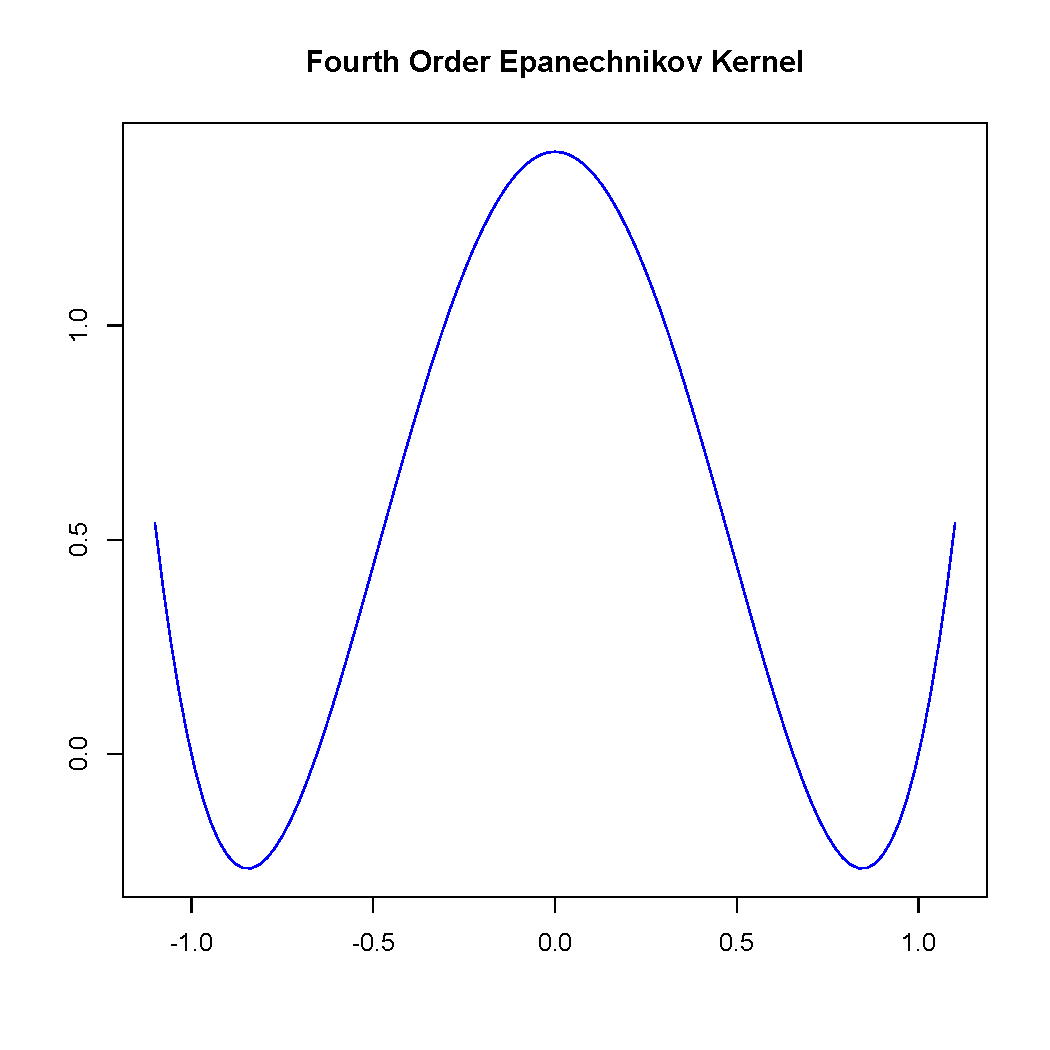
\includegraphics[width = 0.6\textwidth]{p2.pdf}
\end{figure}

\end{enumerate}


\item We begin by deriving the bias of $\hat{F}_n(x) = \frac{1}{n}\sum_{i=1}^{n}\kappa\left(\frac{x-X_i}{h}\right)$

\begin{align*}
\E[\hat{F}_n(x)] &= \frac{1}{n}\sum_{i=1}^{n}\E\left[\kappa\left(\frac{x-X_i}{h}\right)\right]\\
&= \E\left[\kappa\left(\frac{x-W}{h}\right)\right]\\
&= \int_{-\infty}^{\infty}\kappa\left(\frac{x-w}{h}\right)f(w)dw\\
&\overset{z-sub}{=}h\int_{-\infty}^{\infty}\kappa(z)f(x-zh)dz
\end{align*}

We now look integrate by parts with $u = \kappa(z)= \int_{-\infty}^zK(x)dx$ and $dv = f(z-zh)dz$. By the Fundamental Theorem of Calculus we see $du = (K(z) - K(-\infty))dz = K(z)dz$ because $K$ is a density function. Moreover, $v = -\frac{1}{h}F_n(x-zh)$. This gives 

\begin{align*}
h\int_{-\infty}^{\infty}\kappa(z)f(x-zh)dz &= h\bigg[-\frac{1}{h}\kappa(z)F_n(x-zh)\Big\vert_{-\infty}^{\infty} +\frac{1}{h} \int_{-\infty}^{\infty}F_n(x-zh)K(z)dz\bigg]\\
&=  -\kappa(\infty)F_n(-\infty) + \kappa(-\infty)F(\infty) +\int_{-\infty}^{\infty}F_n(x-zh)K(z)dz
\end{align*}

Notice that $F(-\infty) = 0$ and $\kappa(-\infty) = 0$ so the first term drops out completely. This gives 

\begin{align*}
\int_{-\infty}^{\infty}F_n(x-zh)K(z)dz &\overset{Taylor}{=}\int_{-\infty}^{\infty}K(z)\Big\{F_n(x) - zhf(x) + \frac{z^2h^2}{2}f'(x) + o(h^2)\Big\} dz\\
&= F_n(x) + \frac{h^2}{2}f'(x)\mu_2(K) + o(h^2)
\end{align*}

Therefore we see the approximate bias is given by $$\frac{h^2}{2}\mu_2(K)f'(x) +o(h^2)$$ Now we calculate the variance of our estimator 

\begin{align*}
Var(\hat{F}_n(x)) &= \frac{1}{n^2}\sum_{i=1}^{n}Var\left[\kappa\left(\frac{x - X_i}{h}\right)\right]\\
&= \frac{1}{n}\left[\E\bigg[\kappa^2\left(\frac{x-W}{h}\right)\bigg] - \bigg[\E\left(\kappa\left(\frac{x-W}{h}\right)\right)\bigg]^2\right]\\
&= \frac{1}{n}\left[\E\bigg[\kappa^2\left(\frac{x-W}{h}\right)\bigg] - \bigg[F_n(x) + O(h^2)\bigg]^2\right]\\
&= \frac{1}{n}\left[\bigg(\int_{-\infty}^{\infty}\kappa^2\left(\frac{x-w}{h}\right)f(w)dw\bigg) - \bigg[F_n(x) + O(h^2)\bigg]^2\right]\\
&\overset{z-sub}{=} \frac{1}{n}\left[\bigg(h\int_{-\infty}^{\infty}\kappa^2(z)f(x - zh)dz\bigg) - \bigg[F_n(x) + o(h)\bigg]^2\right]\\
\end{align*}

Focusing on the first integral, we can again integrate by parts with $u = \kappa^2(z)$ and $dv = f(x-zh)dz$. These values correspond to $du = 2\kappa(z)K(z)dz$ (as above) and $v = -\frac{1}{h}F_{n}(x-zh)$. Using this, we see 

\begin{align*}
h\int_{-\infty}^{\infty}\kappa^2(z)f(x - zh)dz &= -\kappa^2(z)F_n(x-zh)\Big|_{-\infty}^{\infty} + \int_{-\infty}^{\infty}2\kappa(z)K(z)F_n(x-zh)dz\\
&= -\kappa(-\infty)F_n(\infty) + \kappa(\infty)F_n(-\infty) + \int_{-\infty}^{\infty}2\kappa(z)K(z)F_n(x-zh)dz\\
&= \int_{-\infty}^{\infty}2\kappa(z)K(z)F_n(x-zh)dz\\
&\overset{Taylor}{=}\int_{-\infty}^{\infty}2\kappa(z)K(z)\Big\{F_n(x) - zhf(z) + o(h)\Big\}dz\\
&= F_n(x)\int_{-\infty}^{\infty}2\kappa(z)K(z)dz - hf(x)\theta + o(h)\\
&= F_n(x) - hf(x)\theta + o(h)
\end{align*}

Here we used the fact that $$\int_{-\infty}^{\infty} 2\kappa(u)K(u)du = \kappa(u)^2\big\vert_{-\infty}^{\infty} = \kappa(\infty) - \kappa(-\infty) = 1 - 0 = 1$$ Plugging this into the equation above we see 
\begin{align*}
Var(\hat{F}_n(x)) &= \frac{1}{n}\left[F_n(x)-hf(x)\theta + o(h)- \bigg[F_n(x) + o(h)\bigg]^2\right]\\
&=\frac{1}{n}\left[F_n(x)-hf(x)\theta + o(h)- F_n^2(x) + o(h)\right]\\
&= \frac{F_n(x)(1-F_n(x))}{n} - \frac{h}{n}f(x)\theta + o(\frac{h}{n})\\
&= \frac{\sigma^2_F(x)}{n} - \frac{h}{n}f(x)\theta + o(\frac{h}{n})
\end{align*}

This yields the mean squared error as $$MSE = \frac{\sigma^2_F(x)}{n} - \frac{h}{n}f(x)\theta + o(\frac{h}{n}) + \frac{h^4}{4}\mu_2^2(K)f'(x)^2 + o(h^4)$$ and now the MISE as 
\begin{align*}
MISE &= \int MSE \\
&= \int \frac{\sigma^2_F(x)}{n} - \frac{h}{n}f(x)\theta + o(\frac{h}{n}) + \frac{h^4}{4}\mu_2^2(K)f'(x)^2 + o(h^4) dx\\
&= \frac{1}{n}\int \sigma_F^2(x)dx - \frac{h}{n}\int \theta f(x)dx + o(\frac{h}{n}) +\frac{h^4}{4}\mu_2^2(K)\int f'(x)^2dx +o(h^4)\\
&= \frac{1}{n}C_0 - \frac{h}{n}C_1 + h^4C_2
\end{align*}

Now minimizing MISE with respect to $h$ we can find $h_{MISE}$. 

\begin{align*}
\frac{\partial}{\partial h} MISE &= \frac{\partial}{\partial h}\left(\frac{1}{n}C_0 - \frac{h}{n}C_1 + h^4C_2\right) =  -\frac{1}{n}C_1 +h^3C_2\\
\end{align*}

This corresponds to $$h_{MISE} = \Big[\frac{C_1}{nC_2}\Big]^{1/3} =  \Big[\frac{\int \theta f(x)dx}{n\mu_2^{2}(K)\int f'(x)^2dx}\Big]^{1/3} = O(n^{-1/3})$$
Therefore, for $h_{MISE}$ we have an improved rate of convergence given by $$MISE(h_{MISE}) = C_1 n^{-4/3} + Cn^{-4/3} = o(n^{-4/3})$$

Now, we calculate $\theta$ for the Epanechnikov kernel. First we find $\kappa(\cdot)$. 

$$\kappa(u) = \int_{-\infty}^{u}\frac{3}{4}(1-t^2)I_{[-1,1]}(t)dt= \frac{3}{4}\int_{-1}^{u}(1-t^2) = \frac{3}{4}\Big[t-t^3/3\Big]_{-1}^{u} = \frac{1}{4}(-u^3 + 3u + 2)$$
\begin{align*}
\theta &= \int_{-\infty}^{\infty} 2u\kappa(u)K(u)du\\
&= \frac{3}{8}\int_{-1}^{1}u(1-u^2)(-u^3 +3u+2)du\\
&=\frac{3}{8}\int_{-1}^{1}(u^6 -4u^4 -2u^3 + 3u^2 +2u)du\\
&= \frac{3}{8}\left(\frac{u^7}{7}-\frac{4u^5}{5}-\frac{u^4}{2}+u^3 + u^2\right)_{-1}^{1}\\
&= \frac{3}{8}\left(\frac{59}{70} - \frac{11}{70}\right)\\
&= \frac{9}{35}>0
\end{align*}


\item I implemented a CDF kernel estimator using the Epanechnikov. Pictured below is the constant (histogram) estimator of the CDF as well as the kernel estimator with $h =0.25, 0.5, 0.75$.  For implementation details, see the code attached. 


\begin{figure}[h]
\centering
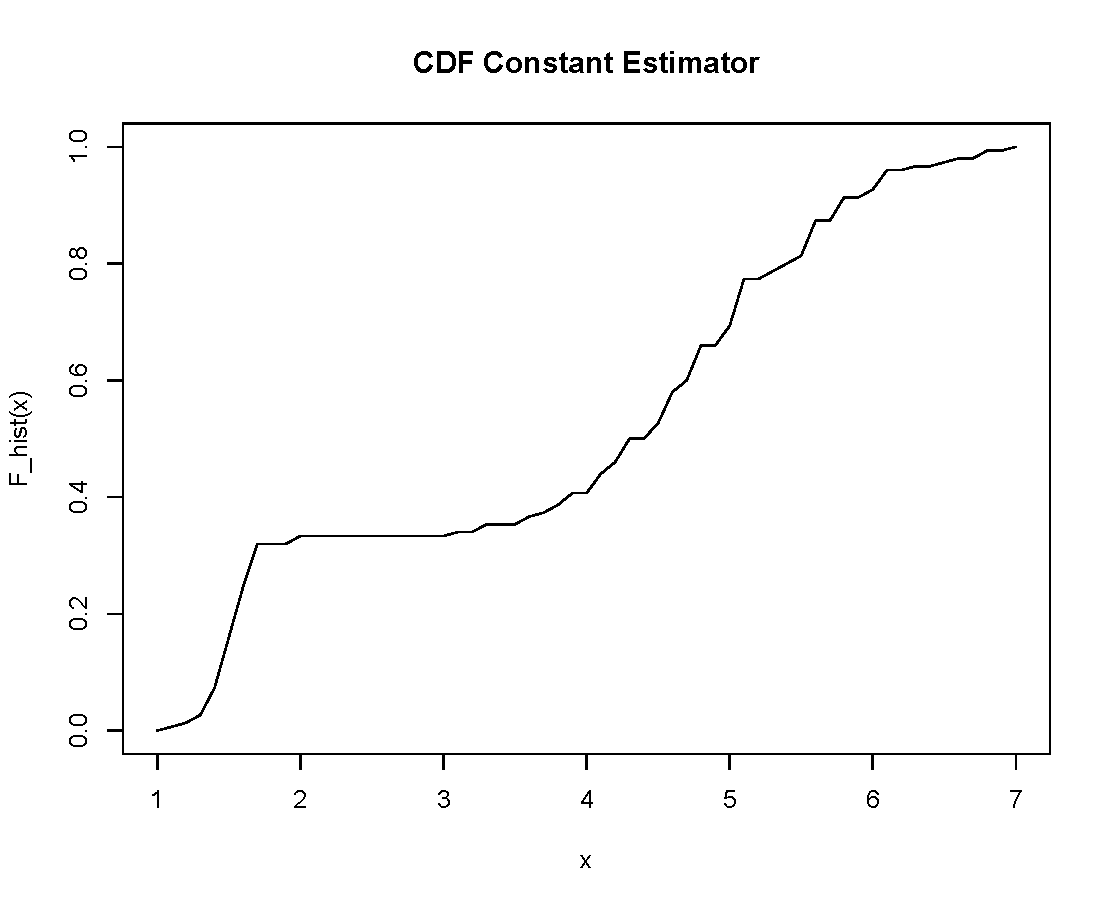
\includegraphics[width = 0.45\textwidth]{p4.pdf}
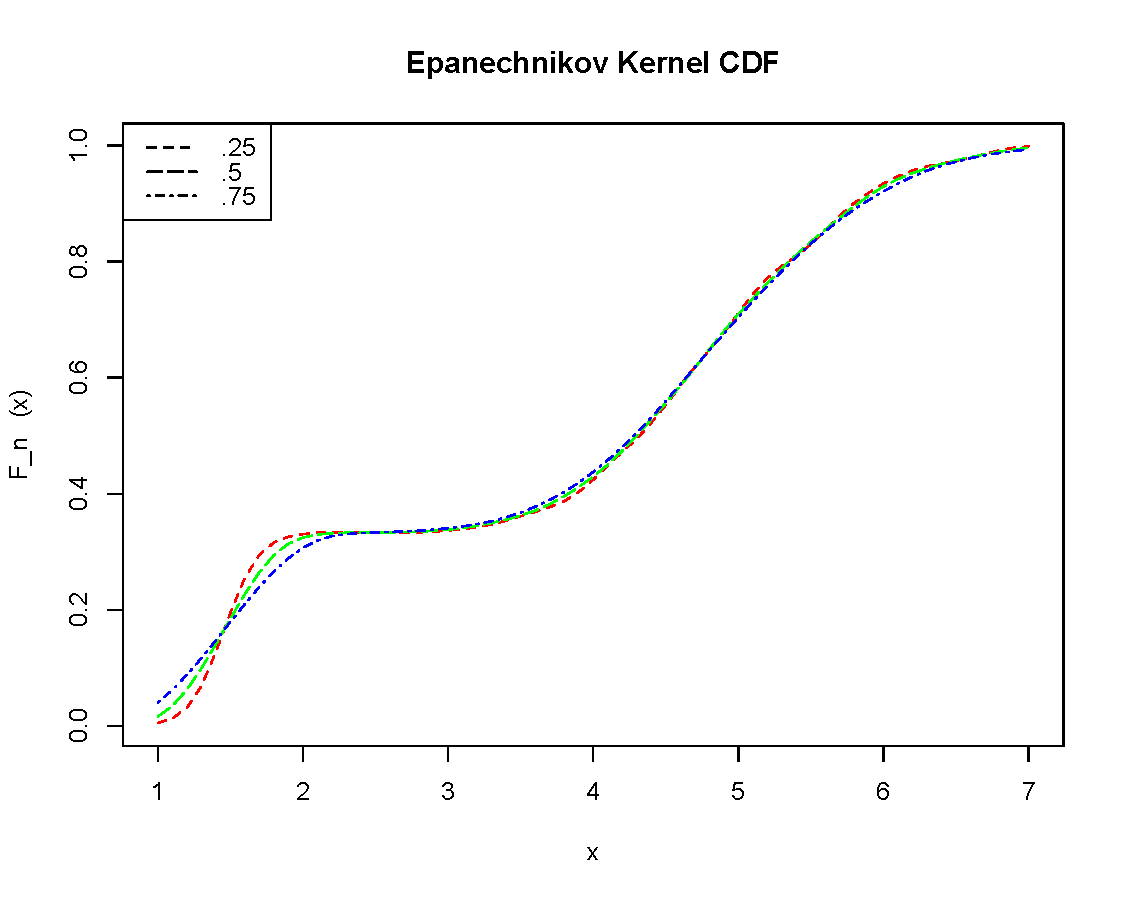
\includegraphics[width = 0.45\textwidth]{p3.pdf}
\end{figure}

\end{enumerate}
\end{document} 

